\documentclass[../main.tex]{subfiles}

\begin{document}

\justifying

\section{Directory: 2026-02-05-140904}

\paragraph{Objetivo} Analizar la tabulación del potencial de interacción entre patches $U_\mathrm{patch}$ en LAMMPS.

\subsection{Simulation description}

Se coloca una partícula en el centro de la caja de simulación, \(\vec{r}_1 = (0,0,0)\).
Se coloca una segunda partícula a una distancia de \num{0.75} de la partícula central, \(\vec{r}_2 = (-0.75,0,0)\).
Usando el comando \verb|fix move| se mueve la segunda partícula a velocidad constante de \num{0.1}, \(\vec{v}_2 = (0.1,0,0)\), hacia el centro de la caja.
El paso temporal es de \num{1d-3}.
El número de pasos es \num{4500}, obteniendo una simulación de \num{4.5} unidades temporales.

\subsection{Resultados}

\begin{figure}[ht]
    \centering
    
\includegraphics[width=\textwidth]{../Figures/2026-02-05-140904/fig_comp.png}
    \caption{Evolución temporal de las componentes de la posición de cada una de las partículas.
    En el panel superior es la componente $x$ de cada partícula y en el panel inferior es la componente $y$ de cada partícula a lo largo de la simulación.}\label{fig:1_componentes}
\end{figure}

\newpage

\begin{figure}[ht]
    \centering
    
\includegraphics[width=0.8\textwidth]{../Figures/2026-02-05-140904/fig_pot.png}
    \caption{Evolución temporal de la energía potencial en cada partícula y la evolución temporal de la distancia entre partículas.
    En el panel de arriba es la evolución temporal de la partícula qué está en el centro y en el panel de abajo es la evolución temporal de la energía potencial de la partícula que se está acercando.
    En el panel de en medio es la evolución temporal de la distancia entre partículas.}\label{fig:2_Upotpart}
\end{figure}

\hfill

\begin{figure}[ht]
    \centering
    
\includegraphics[width=0.8\textwidth]{../Figures/2026-02-05-140904/fig_potComp.png}
    \caption{Comparación de la energía potencial entre la simulación y la forma algebráica.
    \(U_{\mathrm{sim}}\) es la energía potencial que da LAMMPS.
    \(U_{\mathrm{eval}}\) es la energía potencial que sale de evaluar el potencial con la distancia obtenida a través de los datos de la simulación.
    \(U_{\mathrm{ref}}\) es el potencial de interacción evaluado con un dominio creado a parte.}\label{fig:3_UpotComp}
\end{figure}


\newpage

\subsection{Comentarios/Análsis}

\ldots Éxito parcial? 
En términos generales, por la figura \ref{fig:3_UpotComp} se puede decir que la tabulación está parcialmente correcta.
Tiene la forma del pozo potencial, pero el pozo de potencial es mayor con respecto a la definición.

Lo que no logro comprender, son los datos que encuentro en el \verb|dump|.
Creando un zoom de la figura \ref{fig:1_componentes} en las primeras iteraciones (\ref{fig:4_componentes}) podemos obeservar que la partícula \emph{regresa} periódicamente a valores cercanos a su posición original.
No entiendo porque hace eso.

\begin{marginfigure}
    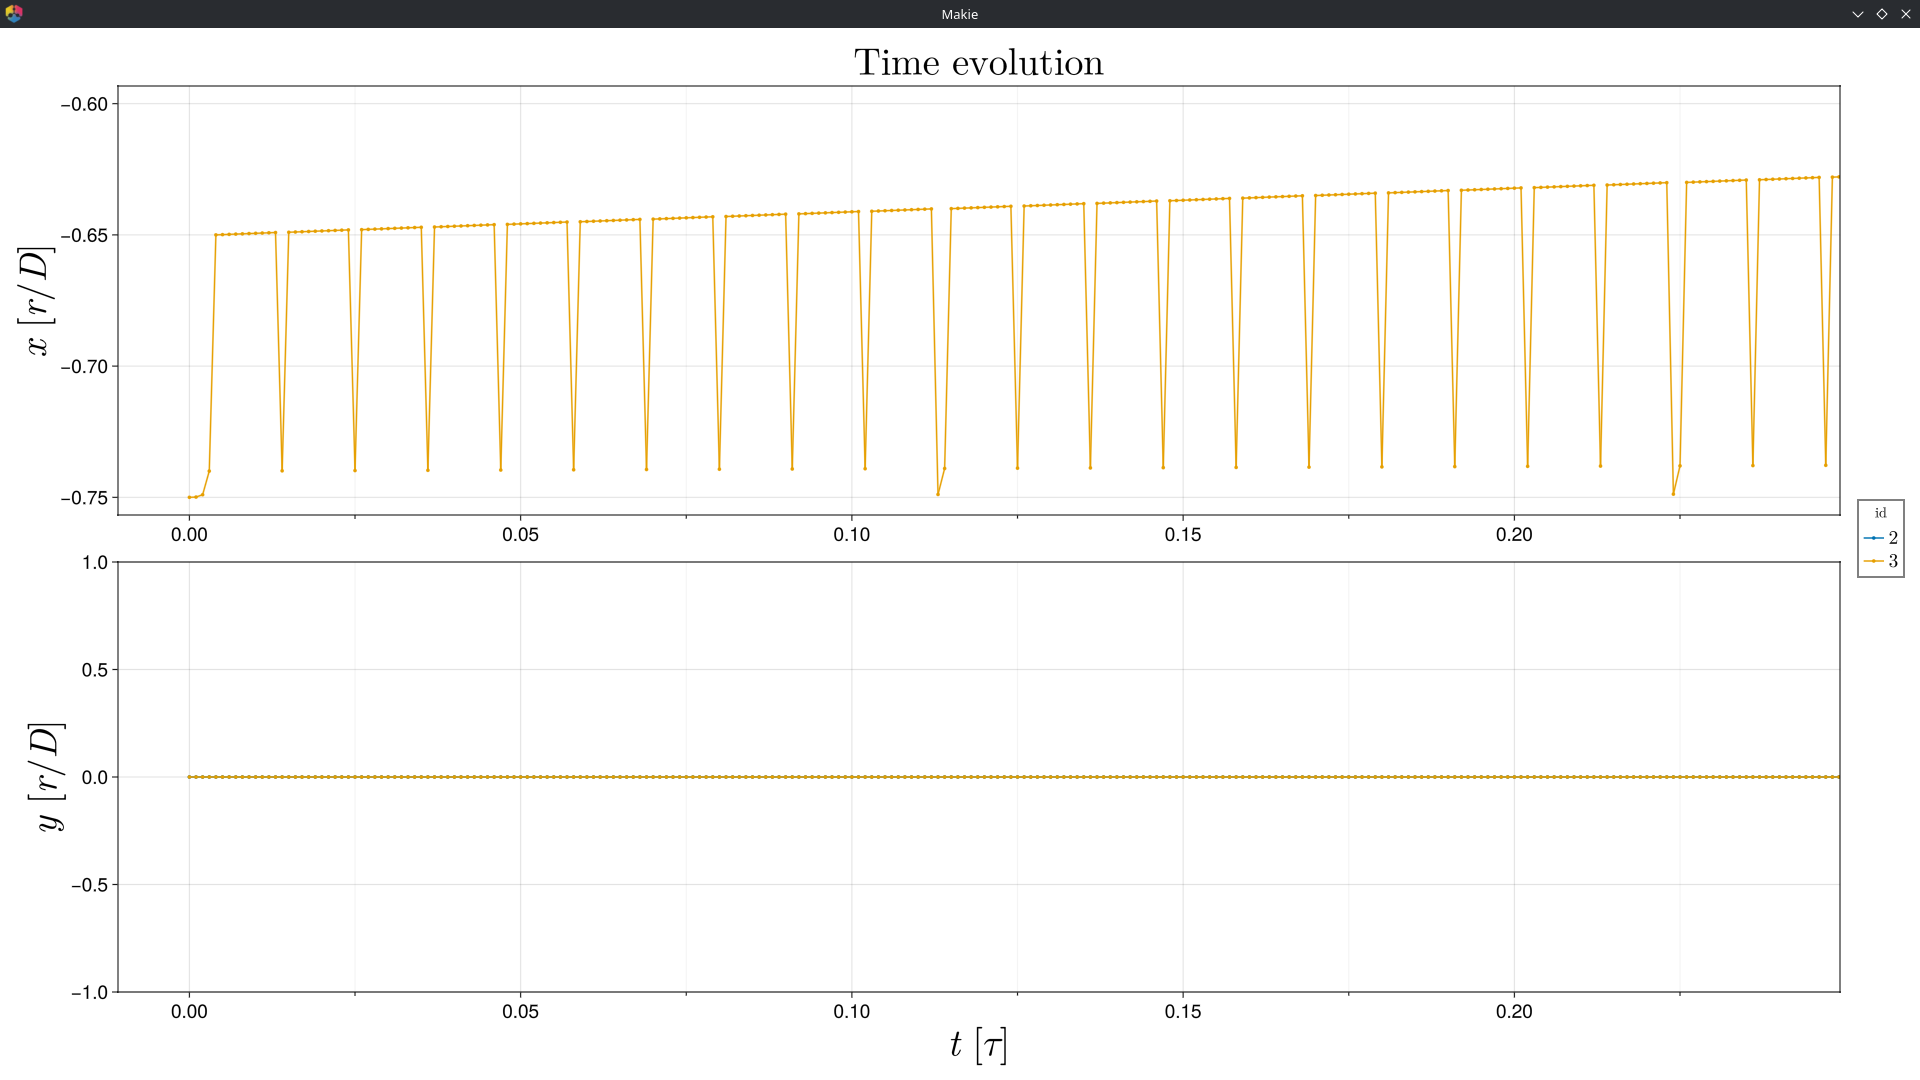
\includegraphics[width=\textwidth]{../Figures/2026-02-05-140904/fig_comp_zoom.png}
    \caption{Acercamiento de la figura~\ref{fig:1_componentes}.}\label{fig:4_componentes}
\end{marginfigure}

El código que configura el movimiento está declarado de la siguiente manera:
\begin{code}
# RUN SIMULATION
timestep ${tstep}
fix movePA PAm move linear 0.1 0.0 0.0
run ${steps}
\end{code}
Fin.

Peor aún, en la figura~\ref{fig:1_componentes}, por el segundo $\approx$\num{3.8} hay una discontinuidad que no sé porque está.
Lo peor de todo es que cuando analizo la información del \verb|dump| en ovito, parece que todo va bien: \href{https://youtu.be/L48lPIuFl4U}{https://youtu.be/L48lPIuFl4U}
\begin{marginfigure}
    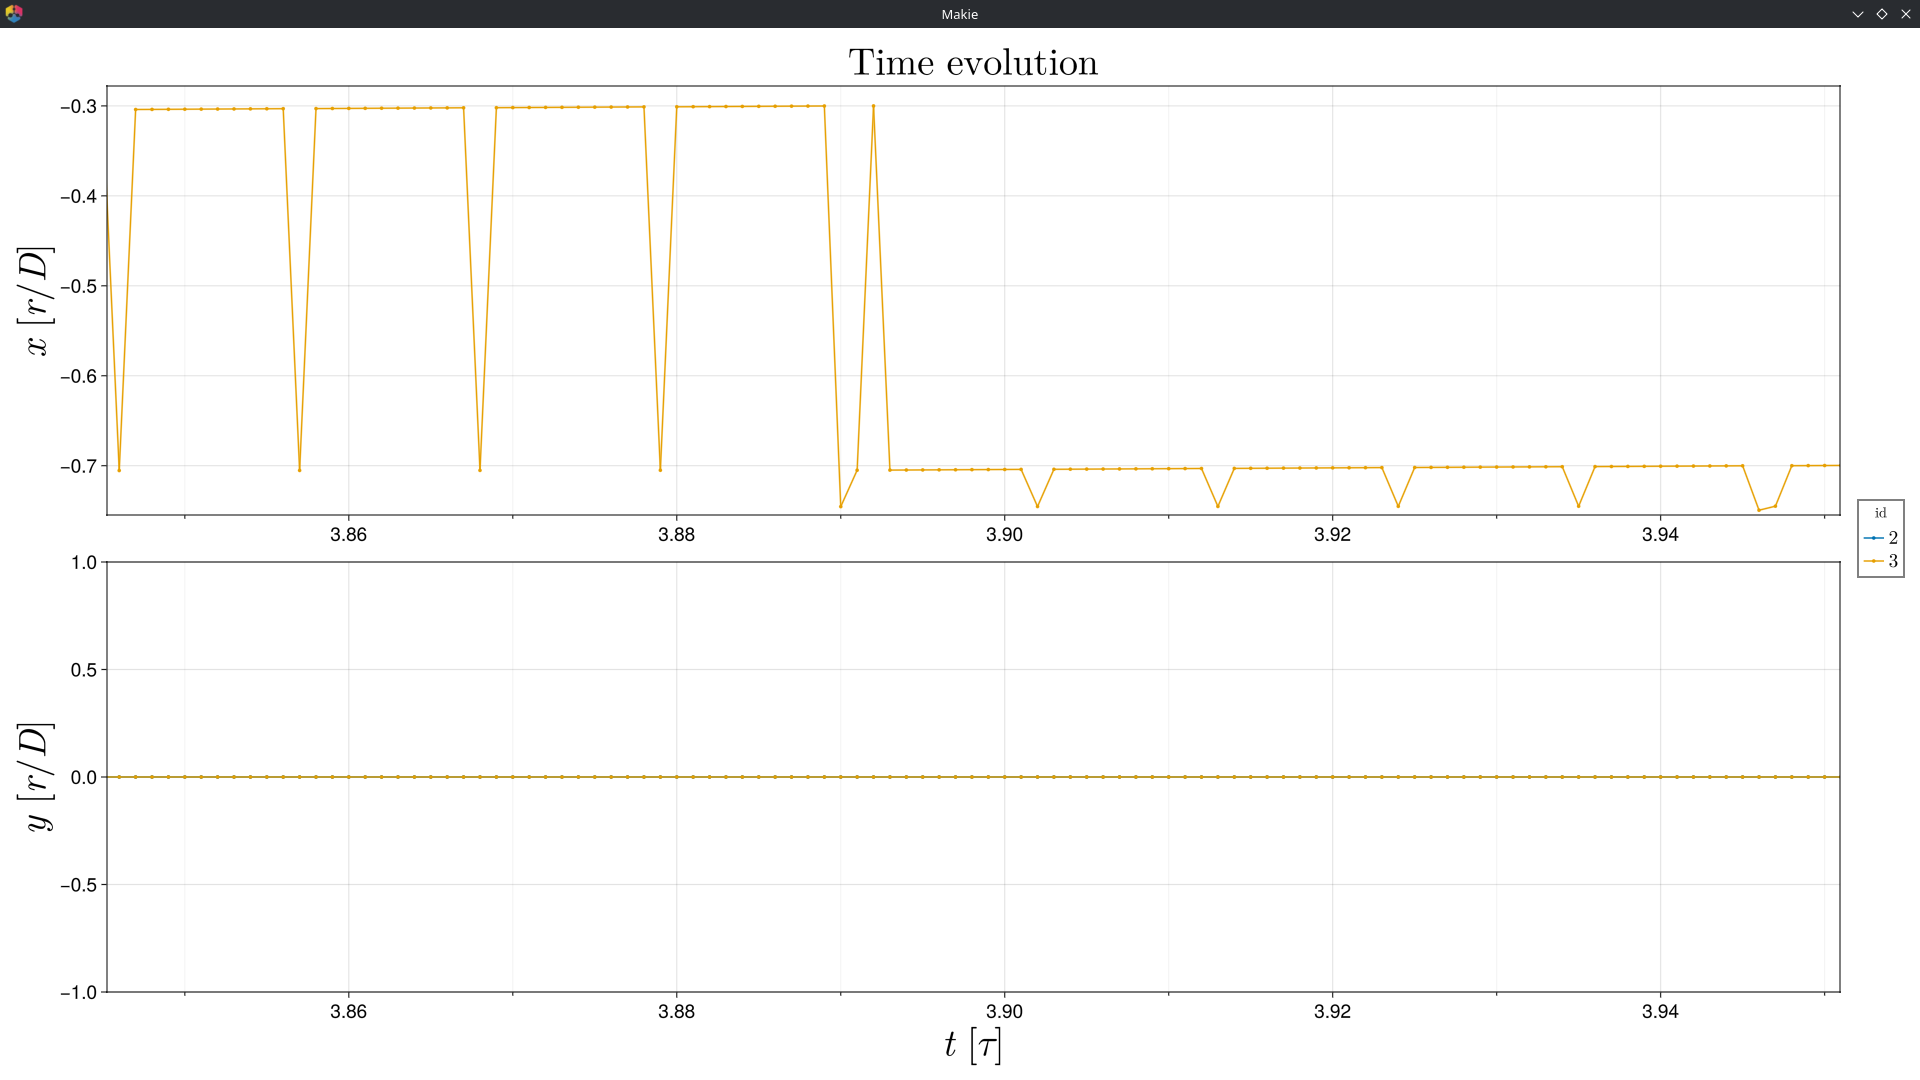
\includegraphics[width=\textwidth]{../Figures/2026-02-05-140904/fig_comp_zoom_2.png}
    \caption{Acercamiento de la figura~\ref{fig:1_componentes}.}\label{fig:5_componentes}
\end{marginfigure}

Viendo con calma, el error está en cómo estoy procesando los archivos \verb|dump|.
Al leer los archivos, la forma en como el sistema operativo ordena los archivos, se tiene un orden que no corresponde a las iteraciones temporales.

\newpage

\subsection{Resultados corregidos}

\begin{figure}[ht]
    \centering
    
\includegraphics[width=0.8\textwidth]{../Figures/2026-02-05-140904/corr/fig_pot.png}
    \caption{Evolución temporal de la energía potencial en cada partícula y la evolución temporal de la distancia entre partículas.
    En el panel de arriba es la evolución temporal de la partícula qué está en el centro y en el panel de abajo es la evolución temporal de la energía potencial de la partícula que se está acercando.
    En el panel de en medio es la evolución temporal de la distancia entre partículas.}\label{fig:2_Upotpartcor}
\end{figure}


%\begin{marginfigure}
%    
\includegraphics[width=\textwidth]{../Figures/2026-02-05-140904/corr/fig_comp.png}
%    \caption{Evolución temporal de las componentes de la posición de cada una de las partículas.
%    En el panel superior es la componente $x$ de cada partícula y en el panel inferior es la componente $y$ de cada partícula a lo largo de la simulación.}\label{fig:1_componentescor}
%\end{marginfigure}


\begin{figure}[ht]
    \centering
    
\includegraphics[width=0.8\textwidth]{../Figures/2026-02-05-140904/corr/fig_potComp.png}
    \caption{Comparación de la energía potencial entre la simulación y la forma algebráica.
    \(U_{\mathrm{sim}}\) es la energía potencial que da LAMMPS.
    \(U_{\mathrm{eval}}\) es la energía potencial que sale de evaluar el potencial con la distancia obtenida a través de los datos de la simulación.
    \(U_{\mathrm{ref}}\) es el potencial de interacción evaluado con un dominio creado a parte.}\label{fig:3_UpotCompcor}
\end{figure}

\subsection{Análisis de datos corregidos}

Pues funcionó la corrección.
Agregé una columna al dataframe asociado a los dumps con el valor del \emph{TimeStep} y después se organizó la base de datos en orden descendiente.

La principal diferencia con el potencial teórico es el mínimo del potencial (figura~\ref{fig:3_UpotCompcor}).

\newpage

\section{Directory: 2026-02-09-104056}

\paragraph{Objetivo} Hacer que el pozo de potencial sea igual a \num{1}.

\subsection{Simulation description}

Se coloca una partícula en el centro de la caja de simulación, \(\vec{r}_1 = (0,0,0)\).
Se coloca una segunda partícula a una distancia de \num{0.75} de la partícula central, \(\vec{r}_2 = (-0.75,0,0)\).
Usando el comando \verb|fix move| se mueve la segunda partícula a velocidad constante de \num{0.1}, \(\vec{v}_2 = (0.1,0,0)\), hacia el centro de la caja.
El paso temporal es de \num{1d-3}.
El número de pasos es \num{4500}, obteniendo una simulación de \num{4.5} unidades temporales.

\subsection{Resultados}

\begin{figure}[!ht]
    \centering
    
\includegraphics[width=0.8\textwidth]{../Figures/2026-02-09-104056/fig_potComp.png}
    \caption{Comparación de la energía potencial entre la simulación y la forma algebráica.
\(U_{\mathrm{sim}}\) es la energía potencial que da LAMMPS.
\(U_{\mathrm{eval}}\) es la energía potencial que sale de evaluar el potencial con la distancia obtenida a través de los datos de la simulación.
\(U_{\mathrm{ref}}\) es el potencial de interacción evaluado con un dominio creado a parte.
}
\end{figure}

\begin{marginfigure}
    
\includegraphics[width=\textwidth]{../Figures/2026-02-09-104056/fig_comp.png}
    \caption{Evolución temporal de las componentes de la posición de cada una de las partículas.
    En el panel superior es la componente $x$ de cada partícula y en el panel inferior es la componente $y$ de cada partícula a lo largo de la simulación.}\label{fig:1_componentes}
\end{marginfigure}

\subsection{Comentarios}

Cambié lo siguiente en el script de la tabulación de LAMMPS: \verb|eps=1.0| y \verb|rmin=sig/2|.
No entiendo porque lammps registra que el pozo de potencial es $0.5$?
Mi intuición es el \emph{style} que tiene el comando \verb|pair_style table| es \emph{linear} y hace es: \emph{For the linear style, the distance R is used to find the 2 surrounding table values from which an energy or force is computed by linear interpolation.}

Mientrás revisaba el código me di cuenta qué la declaración del comando estaba des-actualizado: \verb|table/omp linear 5000000|, cuando debería de marca \num{1000000}.
Cambiaré ese comando para ver si se arregla.
Sí no se arregla, exploraré lo los \emph{style}.

\newpage

\section{Directory: 2026-02-09-111008}

\paragraph{Objetivo} Hacer que el pozo de potencial sea igual a \num{1}.

\subsection{Simulation description}

Se coloca una partícula en el centro de la caja de simulación, \(\vec{r}_1 = (0,0,0)\).
Se coloca una segunda partícula a una distancia de \num{0.75} de la partícula central, \(\vec{r}_2 = (-0.75,0,0)\).
Usando el comando \verb|fix move| se mueve la segunda partícula a velocidad constante de \num{0.1}, \(\vec{v}_2 = (0.1,0,0)\), hacia el centro de la caja.
El paso temporal es de \num{1d-3}.
El número de pasos es \num{4500}, obteniendo una simulación de \num{4.5} unidades temporales.

\subsection{Resultados}

\begin{figure}[!ht]
    \centering
    
\includegraphics[width=0.8\textwidth]{../Figures/2026-02-09-111008/fig_potComp.png}
    \caption{Comparación de la energía potencial entre la simulación y la forma algebráica.
\(U_{\mathrm{sim}}\) es la energía potencial que da LAMMPS.
\(U_{\mathrm{eval}}\) es la energía potencial que sale de evaluar el potencial con la distancia obtenida a través de los datos de la simulación.
\(U_{\mathrm{ref}}\) es el potencial de interacción evaluado con un dominio creado a parte.
}
\end{figure}

\begin{marginfigure}
    
\includegraphics[width=\textwidth]{../Figures/2026-02-09-111008/fig_comp.png}
    \caption{Evolución temporal de las componentes de la posición de cada una de las partículas.
    En el panel superior es la componente $x$ de cada partícula y en el panel inferior es la componente $y$ de cada partícula a lo largo de la simulación.}\label{fig:1_componentes}
\end{marginfigure}

\subsection{Comentarios}

Pues parece que no cambio.
Re-leyendo la documentación, me encontré con lo siguiente: \emph{This means that if you want the interpolation tables of length Ntable to match exactly what is in the tabulated file (with effectively no preliminary interpolation), you should set Ntable = Nfile, and use the “RSQ” or “BITMAP” parameter.}
Usaré el \emph{RSQ} para la siguiente simulación.

\newpage

\section{Directory: 2026-02-09-113140}

\paragraph{Objetivo} Hacer que el pozo de potencial sea igual a \num{1}.

\subsection{Simulation description}

Se coloca una partícula en el centro de la caja de simulación, \(\vec{r}_1 = (0,0,0)\).
Se coloca una segunda partícula a una distancia de \num{0.75} de la partícula central, \(\vec{r}_2 = (-0.75,0,0)\).
Usando el comando \verb|fix move| se mueve la segunda partícula a velocidad constante de \num{0.1}, \(\vec{v}_2 = (0.1,0,0)\), hacia el centro de la caja.
El paso temporal es de \num{1d-3}.
El número de pasos es \num{4500}, obteniendo una simulación de \num{4.5} unidades temporales.

\subsection{Resultados}

\begin{figure}[!ht]
    \centering
    
\includegraphics[width=0.8\textwidth]{../Figures/2026-02-09-113140/fig_potComp.png}
    \caption{Comparación de la energía potencial entre la simulación y la forma algebráica.
\(U_{\mathrm{sim}}\) es la energía potencial que da LAMMPS.
\(U_{\mathrm{eval}}\) es la energía potencial que sale de evaluar el potencial con la distancia obtenida a través de los datos de la simulación.
\(U_{\mathrm{ref}}\) es el potencial de interacción evaluado con un dominio creado a parte.
}
\end{figure}

\begin{marginfigure}
    
\includegraphics[width=\textwidth]{../Figures/2026-02-09-113140/fig_comp.png}
    \caption{Evolución temporal de las componentes de la posición de cada una de las partículas.
    En el panel superior es la componente $x$ de cada partícula y en el panel inferior es la componente $y$ de cada partícula a lo largo de la simulación.}\label{fig:1_componentes}
\end{marginfigure}

\subsection{Comentarios}

Se configuró de siguiente manera la tabla: \verb|N 1000000 RSQ 0.04 0.8|
Si mejoró la parte repulsiva, pero no entiendo porque hay una traslación horizontal y el pozo de potencial no mejoró.
Cambiaré el \emph{style} a \verb|bitmap|

\newpage

\section{Directory: 2026-02-09-114621}

\paragraph{Objetivo} Hacer que el pozo de potencial sea igual a \num{1}.

\subsection{Simulation description}

Se coloca una partícula en el centro de la caja de simulación, \(\vec{r}_1 = (0,0,0)\).
Se coloca una segunda partícula a una distancia de \num{0.75} de la partícula central, \(\vec{r}_2 = (-0.75,0,0)\).
Usando el comando \verb|fix move| se mueve la segunda partícula a velocidad constante de \num{0.1}, \(\vec{v}_2 = (0.1,0,0)\), hacia el centro de la caja.
El paso temporal es de \num{1d-3}.
El número de pasos es \num{4500}, obteniendo una simulación de \num{4.5} unidades temporales.

\subsection{Resultados}

\begin{figure}[!ht]
    \centering
    
\includegraphics[width=0.8\textwidth]{../Figures/2026-02-09-114621/fig_potComp.png}
    \caption{Comparación de la energía potencial entre la simulación y la forma algebráica.
\(U_{\mathrm{sim}}\) es la energía potencial que da LAMMPS.
\(U_{\mathrm{eval}}\) es la energía potencial que sale de evaluar el potencial con la distancia obtenida a través de los datos de la simulación.
\(U_{\mathrm{ref}}\) es el potencial de interacción evaluado con un dominio creado a parte.
}
\end{figure}

\begin{marginfigure}
    
\includegraphics[width=\textwidth]{../Figures/2026-02-09-114621/fig_comp.png}
    \caption{Evolución temporal de las componentes de la posición de cada una de las partículas.
    En el panel superior es la componente $x$ de cada partícula y en el panel inferior es la componente $y$ de cada partícula a lo largo de la simulación.}\label{fig:1_componentes}
\end{marginfigure}

\subsection{Comentarios}

Pues quedó igual.
\verb|pair_style hybrid/overlay zero 0.0 table/omp bitmap 20 threebody/table|.
Donde $M=20$ y $N=2^M$.
Intentaré con la opción de \emph{lookup}.

\newpage

\section{Directory: 2026-02-09-115253}

\paragraph{Objetivo} Hacer que el pozo de potencial sea igual a \num{1}.

\subsection{Simulation description}

Se coloca una partícula en el centro de la caja de simulación, \(\vec{r}_1 = (0,0,0)\).
Se coloca una segunda partícula a una distancia de \num{0.75} de la partícula central, \(\vec{r}_2 = (-0.75,0,0)\).
Usando el comando \verb|fix move| se mueve la segunda partícula a velocidad constante de \num{0.1}, \(\vec{v}_2 = (0.1,0,0)\), hacia el centro de la caja.
El paso temporal es de \num{1d-3}.
El número de pasos es \num{4500}, obteniendo una simulación de \num{4.5} unidades temporales.

\subsection{Resultados}

\begin{figure}[!ht]
    \centering
    
\includegraphics[width=0.8\textwidth]{../Figures/2026-02-09-115253/fig_potComp.png}
    \caption{Comparación de la energía potencial entre la simulación y la forma algebráica.
\(U_{\mathrm{sim}}\) es la energía potencial que da LAMMPS.
\(U_{\mathrm{eval}}\) es la energía potencial que sale de evaluar el potencial con la distancia obtenida a través de los datos de la simulación.
\(U_{\mathrm{ref}}\) es el potencial de interacción evaluado con un dominio creado a parte.
}
\end{figure}

\begin{marginfigure}
    
\includegraphics[width=\textwidth]{../Figures/2026-02-09-115253/fig_comp.png}
    \caption{Evolución temporal de las componentes de la posición de cada una de las partículas.
    En el panel superior es la componente $x$ de cada partícula y en el panel inferior es la componente $y$ de cada partícula a lo largo de la simulación.}\label{fig:1_componentes}
\end{marginfigure}

\subsection{Comentarios}

No entiendo.
Aunque consistentemente el se corta en \num{0.6}.
Voy a cambiar el cutoff cuando se asigna el potencial a un tipo de partícula.

\newpage

\section{Directory: 2026-02-09-115723}


\paragraph{Objetivo} Hacer que el pozo de potencial sea igual a \num{1}.

\subsection{Simulation description}

Se coloca una partícula en el centro de la caja de simulación, \(\vec{r}_1 = (0,0,0)\).
Se coloca una segunda partícula a una distancia de \num{0.75} de la partícula central, \(\vec{r}_2 = (-0.75,0,0)\).
Usando el comando \verb|fix move| se mueve la segunda partícula a velocidad constante de \num{0.1}, \(\vec{v}_2 = (0.1,0,0)\), hacia el centro de la caja.
El paso temporal es de \num{1d-3}.
El número de pasos es \num{4500}, obteniendo una simulación de \num{4.5} unidades temporales.

\subsection{Resultados}

\begin{figure}[!ht]
    \centering
    
\includegraphics[width=0.8\textwidth]{../Figures/2026-02-09-115723/fig_potComp.png}
    \caption{Comparación de la energía potencial entre la simulación y la forma algebráica.
\(U_{\mathrm{sim}}\) es la energía potencial que da LAMMPS.
\(U_{\mathrm{eval}}\) es la energía potencial que sale de evaluar el potencial con la distancia obtenida a través de los datos de la simulación.
\(U_{\mathrm{ref}}\) es el potencial de interacción evaluado con un dominio creado a parte.
}
\end{figure}

\begin{marginfigure}
    
\includegraphics[width=\textwidth]{../Figures/2026-02-09-115723/fig_comp.png}
    \caption{Evolución temporal de las componentes de la posición de cada una de las partículas.
    En el panel superior es la componente $x$ de cada partícula y en el panel inferior es la componente $y$ de cada partícula a lo largo de la simulación.}\label{fig:1_componentes}
\end{marginfigure}

\subsection{Comentarios}

Se arregló lo del \emph{cut off}, pero no entiendo porque tiene una traslación horizontal y el pozo de potencial no es igual a \num{1}.


Graficar el potencial total, no por partícula.
Comparar con las fuerzas.
A ver que pasa con tres partículas.



\newpage

\section{Directory: }

\end{document}
